\documentclass[10pt,a4paper]{article}
\usepackage{rpgcover}
\usepackage{illustrated-panel}
\usepackage{longtable,booktabs}
\usepackage{float}
\usepackage{multicol}
\usepackage{fancyvrb}
\usepackage{wrapfig}
\usepackage{needspace}
\usepackage{titlesec}
\titleformat{\subsection}{\normalfont\Large\bfseries\color{rpgbrown}}{}{0pt}{}
\titlespacing*{\subsection}{0pt}{12pt plus 2pt}{5pt}
\titleformat{\subsubsection}{\normalfont\normalsize\bfseries\color{rpgbrown}}{}{0pt}{}
\titlespacing*{\subsubsection}{0pt}{10pt plus 2pt}{4pt}
\usepackage{etoolbox}
% Stat boxes never start in the last lines of a page, where they would split after their title.
\BeforeBeginEnvironment{rpgnote}{\par\needspace{8\baselineskip}}
\pretocmd{\subsection}{\needspace{5\baselineskip}}{}{}
\pretocmd{\subsubsection}{\needspace{4\baselineskip}}{}{}
\setcounter{tocdepth}{1}
\clubpenalty=10000
\widowpenalty=10000
\displaywidowpenalty=10000
\interlinepenalty=100
\emergencystretch=1.2em
\newcommand{\HHInlineFigure}[3]{%
  \begin{center}\includegraphics[width=#2\linewidth,height=70mm,keepaspectratio]{assets/hollow-hearth/#1.jpg}%
  \par\vspace{2pt}{\footnotesize\itshape\color{rpgbrown}#3\par}\end{center}}
% Scene-opening illustrations float: here when they fit, otherwise at the foot of the next page.
% They never narrow a read-aloud box or leave a gap at the bottom of a page.
\newcommand{\HHSceneArt}[2]{%
  \begin{figure}[!hb]\centering\includegraphics[width=.62\linewidth,height=58mm,keepaspectratio]{assets/hollow-hearth/#1.jpg}%
  \par\vspace{2pt}{\footnotesize\itshape\color{rpgbrown}#2\par}\end{figure}}
% Full-page maps float to the next free page instead of ending the current page early.
\newcommand{\HHSceneMap}[3]{%
  \begin{figure}[p]\centering
    {\Large\bfseries\color{rpgbrown}#2\par}\vspace{6mm}%
    \includegraphics[width=.96\linewidth,height=190mm,keepaspectratio]{assets/hollow-hearth/#1.jpg}\par\vspace{4mm}%
    {\small\itshape\color{rpgbrown}#3\par}%
  \end{figure}}
\newcommand{\HHContents}{%
  \clearpage\thispagestyle{rpg}
  \vspace*{10mm}\begin{center}{\fontsize{27}{31}\selectfont\bfseries TABLE OF CONTENTS\par}\vspace{9pt}
  {\color{rpgline}\rule{.76\linewidth}{.55pt}}\end{center}\vspace{9mm}
  \begingroup
  \expandafter\def\csname l@section\endcsname##1##2{\csname @dottedtocline\endcsname{1}{0em}{4em}{\bfseries ##1}{##2}}%
  \csname @starttoc\endcsname{toc}\endgroup
  \vspace{5mm}
  \begin{center}
\includegraphics[height=68mm,width=.59\linewidth,keepaspectratio]{assets/hollow-hearth/front-overlay.png}\end{center}
  \vfill
  \begin{center}{\small\itshape An adventure by Jacopo Biscella\par}\vspace{5pt}
  {\footnotesize This adventure is licensed under Creative Commons Attribution-ShareAlike 4.0 International (CC BY-SA 4.0), under the same terms as At the Last Throw. You are free to share and adapt this material, including commercially, provided you credit the author and distribute derivative works under the same license.\par}\end{center}
  \clearpage}
\RPGSetRunningTitle{The Bell of Hollow Hearth}
\RPGSetCoverWordSpace{.78em}
\hypersetup{pdftitle={The Bell of Hollow Hearth — At the Last Throw},pdfauthor={Jacopo Biscella}}
\setlength{\emergencystretch}{2em}
\setcounter{secnumdepth}{-1}
\newcommand{\tightlist}{\setlength{\itemsep}{0pt}\setlength{\parskip}{0pt}}

\newcommand{\HHFrontArt}{assets/hollow-hearth/front-overlay.png}
\newcommand{\HHBackArt}{assets/hollow-hearth/back-overlay.png}
% Existing rpgcover.sty is used unchanged; only an adventure-specific back-cover layout follows.
\newcommand{\HHAdventureBackCover}{%
 \clearpage\pagenumbering{gobble}\RPGCoverPagetrue\thispagestyle{empty}\null
 \begin{tikzpicture}[remember picture,overlay,x=1mm,y=1mm]
  \RPGDrawBackground{\RPGBackBackgroundFile}
  \node[align=center,text=coverink,text width=170mm,inner sep=0pt] at ($(current page.south west)+(105mm,260mm)$)
    {{\RPGCoverTitleFont\fontsize{19}{23}\selectfont THE BELL OF HOLLOW HEARTH}};
  \draw[coverink,line width=.45pt] ($(current page.south west)+(57mm,246mm)$)--($(current page.south west)+(153mm,246mm)$);
  \node[anchor=north,align=left,text=coverink,text width=137mm,inner sep=0pt] at ($(current page.south west)+(105mm,240mm)$)
    {\RPGCoverTextFont\fontsize{10.4}{13.4}\selectfont
    Seven generations ago, a wandering Mystic blessed a bronze bell cast in the forge of a small village built where the king's road ends and the old forest begins. The village took the name Hollow Hearth. The bell, rung at every dusk, kept the Hollow Folk \textemdash{} pale, bark-skinned things that whisper from between the trees \textemdash{} at bay among the roots.};
  \node[anchor=north,align=center,text=coverink,text width=140mm,inner sep=0pt] at ($(current page.south west)+(105mm,197mm)$)
    {\RPGCoverSubtitleFont\fontsize{13}{17}\selectfont Three nights ago, the bell was stolen.\\[4pt]
    The next moonless night is in forty-eight hours.};
  \draw[coverink,line width=.45pt] ($(current page.south west)+(57mm,167mm)$)--($(current page.south west)+(153mm,167mm)$);
  \node[anchor=north,align=left,text=coverink,text width=137mm,inner sep=0pt] at ($(current page.south west)+(105mm,162mm)$)
    {\RPGCoverTextFont\fontsize{9.9}{12.1}\selectfont
    An introductory adventure for At the Last Throw, designed for parties of three or four Protagonists. A single session of two or three hours. Teaches dice tiers, narrative distances, the Wound pool, magic and Backlash, and the moment that gives the game its name.};
  \node[anchor=north,align=center,text=coverink,text width=147mm,inner sep=0pt] at ($(current page.south west)+(105mm,133mm)$)
    {\RPGCoverSubtitleFont\fontsize{10.5}{13.2}\selectfont
     Three approaches. One ending of the group's choosing.\\
     A disgraced knight. A buyer who is not what he seems.\\
     A decision the party will make together.};
  \node[anchor=north,align=center,text=coverink,text width=144mm,inner sep=0pt] at ($(current page.south west)+(105mm,114mm)$)
    {\RPGCoverTextFont\fontsize{10.2}{12.5}\selectfont
     Includes: four maps $\cdot$ five narrative illustrations $\cdot$\\
     a Narrator's quick reference of rules and encounters.};
  \RPGOptionalArtwork{105}{59}{130}{24}{\HHBackArt}
  \filldraw[fill=white,draw=coverink,line width=.55pt]
    ($(current page.south west)+(139mm,25mm)$) rectangle
    ($(current page.south west)+(187mm,55mm)$);
 \end{tikzpicture}
 \clearpage\RPGCoverPagefalse
}
\newcommand{\HHFrontCover}{%
 \clearpage\RPGCoverPagetrue\thispagestyle{empty}\null
 \begin{tikzpicture}[remember picture,overlay,x=1mm,y=1mm]
  \RPGDrawBackground{\RPGFrontBackgroundFile}
  \node[align=center,text=coverink,text width=138mm,inner sep=0pt]
   at ($(current page.south west)+(105mm,248mm)$)
   {\RPGCoverTitleFont\fontsize{16.6}{20.7}\selectfont THE BELL OF\\[1.0mm]HOLLOW HEARTH};
  \node[align=center,text=coverink,text width=135mm,inner sep=0pt]
   at ($(current page.south west)+(105mm,235mm)$)
   {\RPGCoverSubtitleFont\fontsize{9.5}{12}\selectfont An adventure for “At the Last Throw”};
  \RPGOptionalArtwork{105}{119}{150}{138}{\HHFrontArt}
  \node[align=center,text=coverink,text width=124mm,inner sep=0pt]
   at ($(current page.south west)+(105mm,25mm)$)
   {\RPGCoverTextFont\fontsize{12}{15}\selectfont Jacopo Biscella};
 \end{tikzpicture}\clearpage\RPGCoverPagefalse}
\begin{document}
\RPGStartFrontMatter
\HHFrontCover
\HHContents
\RPGStartMainMatter
\RPGChapter{The Bell of Hollow Hearth}
\begin{center}\textit{An introductory adventure for At the Last Throw}\par\smallskip
\small 2--3 hours \textperiodcentered\ 3--4 Protagonists \textperiodcentered\ At least one Fighter \textperiodcentered\ Narrator's edition
\end{center}
\noindent\textit{The four pre-generated character sheets will be provided in a separate PDF, one sheet per Protagonist, using the rulebook character-sheet template.}\par\medskip
\subsection{A Word to the Narrator}\label{a-word-to-the-narrator}

This adventure is a teaching tool first and a story second. Every scene foregrounds a specific pillar of \emph{At the Last Throw} without ever pausing the fiction to lecture. By the time the credits roll, your players will have lived through tier rolls, narrative distances, the Wounds-and-Fatigue pool, the Helping mechanic, and --- if you do your job --- at least one Exertion declared with a shaky hand at exactly the moment the title promises.

The pacing target is roughly:

\begin{itemize}
\tightlist
\item
  30 minutes for character creation and setup \emph{(use the creation rules from the manual, pp. 2--6)}
\item
  35 minutes for \textbf{Scene 1 · The Village} (social investigation)
\item
  40 minutes for \textbf{Scene 2 · The Whispering Wood} (skill challenge + atmosphere)
\item
  60 minutes for \textbf{Scene 3 · The Old Watchtower} (combat climax + resolution)
\item
  10 minutes for \textbf{The Three Questions} and aftermath
\end{itemize}

A reminder that bears repeating: in this game there are no initiative rolls, no fixed turn order, no grid. The maps included with this adventure are spatial anchors for everyone\textquotesingle s imagination --- distances at the table are always \textbf{Close}, \textbf{Near}, \textbf{In Range}, or \textbf{Far}.

\par\vspace{3pt}

\subsection{What This Adventure Teaches}\label{what-this-adventure-teaches}

\begingroup\setlength{\arrayrulewidth}{.34pt}\arrayrulecolor{rpgline}\renewcommand{\arraystretch}{1.32}\rowcolors{2}{rpgshade}{white}\par\smallskip\noindent\begin{tabularx}{\linewidth}{|Y|Y}\hline
\rpghead{Scene} & \rpghead{Mechanics introduced} \\ \hline
The Village & Attribute + Skill rolls; TN for social actions; opposed rolls; Trait and Burden engagement \\ \hline
The Whispering Wood & Helping; Conditions ($-1$ tier); narrative distance bands \\ \hline
The Old Watchtower & Combat; Wounds and Fatigue; Critical; Backlash; \textbf{Exertion}; consequences \\ \hline
\end{tabularx}\arrayrulecolor{black}\endgroup\par\smallskip

If the party includes a Mystic, Scene 3 is also where their first Backlash will likely occur --- let it.

\par\vspace{3pt}

\par\needspace{65mm}\subsection{The Premise}\label{the-premise}

\begin{wrapfigure}{r}{.38\linewidth}\vspace{-5pt}\centering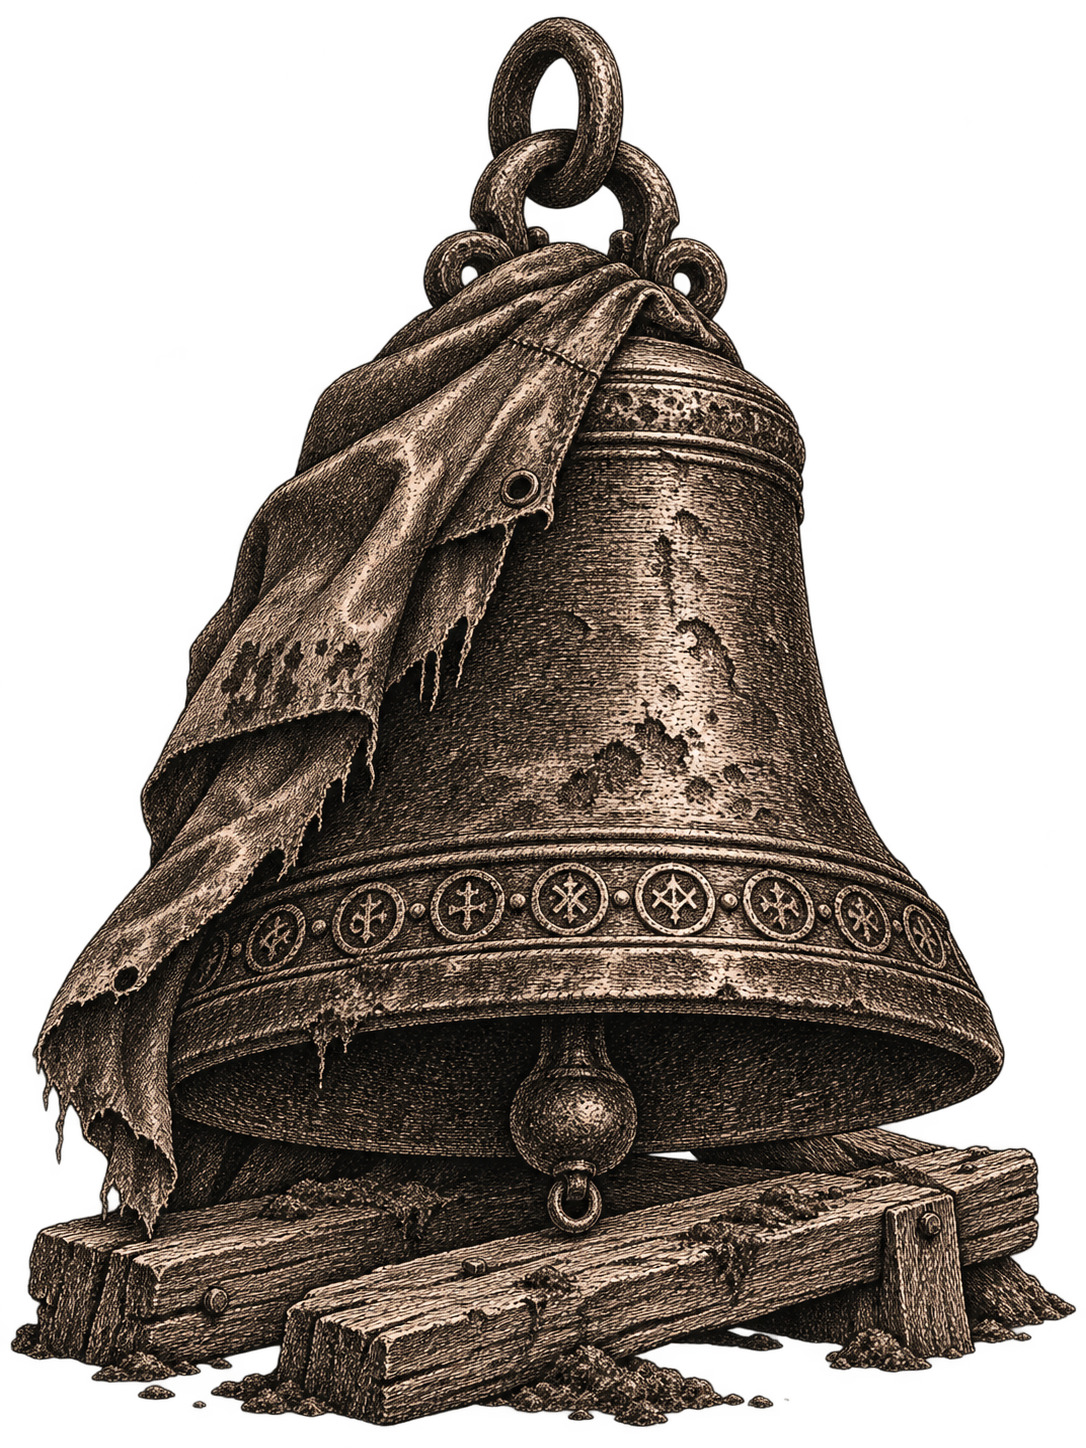
\includegraphics[width=.98\linewidth,height=58mm,keepaspectratio]{assets/hollow-hearth/bell.jpg}\par{\scriptsize\itshape\color{rpgbrown}The stolen bell, wrapped in oilcloth}\vspace{-5pt}\end{wrapfigure}

Seven generations ago, a wandering Mystic named \textbf{Veyl Ashen} blessed a bronze bell cast in the forge of a small settlement built where the King\textquotesingle s road ends and the old forest begins. The settlement took the name \textbf{Hollow Hearth}. The bell, rung at every dusk, kept the \textbf{Hollow Folk} --- pale, bark-skinned things that whisper from between the trees --- back among the roots where they belong.

Three nights ago, the bell was stolen.

A band of brigands led by a deserter named \emph{"Sir"} \textbf{Corwin Vask} descended from the watchtower ruins where they camp, killed the old bellringer\textquotesingle s apprentice, and vanished northward into the wood with the bell wrapped in oilcloth. The villagers buried the boy yesterday morning.

The next moonless night is in \textbf{forty-eight hours}.

That is the clock. After moonset on that night, with no bell to sound at dusk, the Hollow Folk will return to a Hollow Hearth that has forgotten how to defend itself.

\par\vspace{3pt}

\subsection{The Hook}\label{the-hook}

\HHSceneArt{village}{Hollow Hearth at dusk: the empty platform}

Tailor the arrival to the Traits and Burdens your players have written. Some quick prompts:

\begin{itemize}
\tightlist
\item
  A \textbf{Scholar} tracking the lineage of Veyl Ashen through old liturgical records.
\item
  An \textbf{Adventurer} carrying a contract from the next town up the road.
\item
  A \textbf{Mystic} who \emph{felt} the bell go silent from leagues away.
\item
  A \textbf{Fighter} walking off a battlefield they no longer want to be on.
\end{itemize}

Whatever the route, the village mayor, \textbf{Hesta Thrush}, will offer them what little Hollow Hearth has --- coin, hospitality, and a relic kept since the founding (see \emph{Resolution}) --- to bring the bell home.

\begin{quote}
\subsubsection{Read aloud --- Arrival}\label{read-aloud--arrival}

\emph{The road thins to a track, the track to a footpath, and the footpath spills into a clearing of low stone houses with steep slate roofs. A wooden platform stands in the centre of the village square. Empty. Four iron bolts, where something heavy was wrenched away. There is no smoke from the chimneys. There is no one in the square.}

\emph{Then a door opens, and an old woman steps out, and behind her you can hear someone weeping.}
\end{quote}

\par\vspace{3pt}

\HHSceneMap{map-village}{Hollow Hearth: village layout}{The bell platform stands in the square; Hesta, Bram, Vela and the inn are nearby. All village locations: Near.}
\RPGChapter{Scene 1 — The Village}\label{scene-1--the-village}

\textbf{Mechanic focus:} Lore rolls, Skill bonuses, opposed rolls, Trait \& Burden engagement.

There are three people in Hollow Hearth who matter to your investigation. The Protagonists may speak with all three, in any order. Each holds one piece of the picture, and at least one of them is \emph{almost} lying.

\par\smallskip\begin{rpgnote}[fontupper=\normalfont]\textbf{Village NPCs}\par\smallskip
\textbf{Hesta Thrush} \emph{(NPC)} --- Lore Competent. No combat stats; if violence touches her, she is what she appears to be.\par\smallskip
\textbf{Vela Roan} \emph{(NPC)} --- Lore Expert (Herbalism, Survival), Wonder Competent. Will not fight unless cornered.\par\smallskip
\textbf{Old Bram} \emph{(NPC)} --- Lore Competent. Cannot fight any longer.\end{rpgnote}\par\smallskip
Refer to \textbf{the Hollow Hearth village map} for the layout. All village locations are within \textbf{Near} distance of one another.

\subsubsection{Hesta Thrush --- The Mayor}\label{hesta-thrush--the-mayor}

A woman in her sixties, weather-cracked, narrow with grief. Her son left for the war and never came home; she has been mayor for eleven years and knows everyone in the village by middle name.

What she knows freely:

\begin{itemize}
\tightlist
\item
  The brigands came from the \textbf{Old Watchtower}, four hours\textquotesingle{} walk north into the Whispering Wood.
\item
  She offers, as the village\textquotesingle s final reward, a relic from the founding: the \textbf{Blade of Salt} \emph{(manual p. 9)}.
\end{itemize}

What she will lie about:

She knows her cousin \textbf{Marrel} was seen drinking with one of the brigands at the inn the week before the theft. She does not want her cousin hanged for it. A \textbf{Lore roll opposed by Hesta\textquotesingle s Lore (Competent)} catches the discomfort. \textbf{Diplomacy} convinces her to come clean; \textbf{Rhetoric} likewise. \textbf{Intimidation, TN 5} also works, but turns the village against the party for the rest of the adventure.

\begin{quote}
\subsubsection{Trait/Burden hook}\label{traitburden-hook}

A Protagonist whose Burden involves war, lost children, or broken oaths will find Hesta either an ally or a mirror. Lean into it. \emph{"You remind me of him,"} she says, looking at the wrong person.
\end{quote}

\subsubsection{Old Bram --- The Bellringer}\label{old-bram--the-bellringer}

The bellringer, in his eighties, who survived because he was relieving himself in the brambles when the brigands came. The boy who died was his apprentice and his great-nephew. He is angry. Not loud. The other kind.

What he saw:

\begin{itemize}
\tightlist
\item
  Four men. One in armour, one with a longbow, two with daggers.
\item
  The armoured one had a \textbf{white sun stitched on the shoulder of his cloak} --- the heraldry of a knightly order disgraced ten years ago. A \textbf{Lore roll, TN 4 with the History skill} identifies the order as the \textbf{Order of the Pale Sun}, dissolved for "ritual offences" in the wars. Without History, \textbf{TN 5} to dredge up vague memory.
\item
  He believes the bell is alive. He may be right.
\end{itemize}

\subsubsection{Vela Roan --- The Herbalist}\label{vela-roan--the-herbalist}

Forty, sharp, the only person in the village who has been \emph{into} the Whispering Wood and come back. She knows what the Hollow Folk are. She will not say it plainly. She speaks in stories.

What she offers, if asked the right way:

\begin{itemize}
\tightlist
\item
  The "bark-people" come from the roots when no bell rings. She believes one Hollow person is already walking among the villagers in mortal guise.
\item
  She will give a vial of \textbf{distilled nightroot} --- \emph{a notable object: poured on a blade, the next blow inflicts +1 Wound against unnatural creatures; one use only} --- \textbf{if} a Protagonist agrees to bring her a sprig of \textbf{moonsilver flower} from deep in the wood.
\end{itemize}

This last is a side temptation: a chance for a Burden moment if anyone breaks their word later, or a chance for an honourable Trait to be tested. The flower exists. Whether the party finds time for it is up to them.

\subsubsection{Optional · Marrel the Cousin}\label{optional--marrel-the-cousin}

If the Protagonists pursue Hesta\textquotesingle s lie, Marrel can be found at the inn, drinking through his fear. He confirms the brigand he spoke with --- a man named \textbf{Thessik} --- bragged about a buyer who \emph{"pays in northern silver"} coming for the bell. Marrel did not know it would be stolen. \textbf{Intimidation, TN 4} breaks him. \textbf{Diplomacy, TN 4} with a drink also works. \textbf{Commerce, TN 4} if a Scholar wants to talk through what "northern silver" actually means (it is a term used by smugglers crossing the border --- northern silver does not exist, it is a code for fey gold).

\subsubsection{Teaching moment for the Narrator}\label{teaching-moment-for-the-narrator}

When a player declares \emph{"I want to know if she\textquotesingle s lying,"} ask them \textbf{how}. Are they pressing? Watching? Catching her in a contradiction? The \emph{how} determines the Attribute and skill. \textbf{Lore} is the default for reading a person; \textbf{Etiquette} catches her in courtly slips, \textbf{Intimidation} forces her into mistakes, \textbf{Deception} lets you out-lie her into a corner. There is no separate social-combat subsystem. There is just Lore plus a relevant skill against a TN. Same as everything else.

\par\vspace{3pt}

\HHSceneMap{map-forest}{Through the Whispering Wood}{Village below, tower above; the Hollow Folk appear on the bank the party has just left.}

\RPGChapter{Scene 2 — The Whispering Wood}\label{scene-2--the-whispering-wood}

\HHSceneArt{hollow}{A watcher among the trees}

\textbf{Mechanic focus:} Helping mechanic, distance bands, Conditions as -1 tier.

A path of crushed bracken and dropped oilcloth scraps leads north from the village. The Whispering Wood swallows it within fifty paces. The trees here lean inward.

\begin{quote}
\subsubsection{Read aloud --- Entering the Wood}\label{read-aloud--entering-the-wood}

\emph{The light drops a third the moment you cross the treeline. Not from the canopy --- there is no canopy worth the name --- but as if the air itself drinks it. Sound flattens. Footsteps stop carrying. After ten minutes of walking, the only thing you can hear is your own breath and, very far off, what could be wind in branches or could be voices saying something you cannot quite catch.}
\end{quote}

Refer to \textbf{the Whispering Wood journey map} for the layout of the journey from village to watchtower, with the bridge and the Glimpse waypoint marked.

\subsubsection{The Trail · A Survival Challenge}\label{the-trail--a-survival-challenge}

The trail is real but easy to lose. A character with \textbf{Survival} rolls \textbf{TN 4 Dexterity}. A Dex Competent character with the skill rolls 2d6 keep highest; a Dex Expert without the skill rolls the same; a Dex Untrained with no skill rolls 2d6 keep lowest, which is unkind.

This is the perfect moment to introduce \textbf{Helping} \emph{(manual p. 7)}:

\begin{itemize}
\tightlist
\item
  A \textbf{Competent helper} --- one whose own roll on the same task would be at Expert level or higher --- adds \textbf{+1d6} to the lead character\textquotesingle s pool with no penalty.
\item
  An \textbf{Incompetent helper} --- anyone who would roll below Expert level on the same task --- adds \textbf{+1d6} \emph{but raises the TN by one}. A Fighter loudly "helping" the Adventurer track may make things worse.
\end{itemize}

Let the players watch this happen. A Fighter who helps the tracker turns TN 4 into TN 5 --- and then realises the lesson when the trail is lost.

If the trail is lost, an extra hour passes and dusk catches the party in the wood. Everything from that point until sunrise rolls under a \textbf{Condition: -1 tier}.

\subsubsection{The Rotted Bridge}\label{the-rotted-bridge}

The trail crosses a ravine on a single-log bridge that has not been maintained in twenty years. The log will hold one person at a time. Across is fifty feet down to a stream over rocks.

\begin{itemize}
\tightlist
\item
  \textbf{Dex roll, TN 4} to cross safely. With \textbf{Acrobatics}, comfortable.
\item
  A character who falls takes \textbf{2 Wounds} (Combat --- from the rocks). A \textbf{Medicine roll, TN 4}, in-scene, restores 1 Wound (2 on a Critical).
\item
  A rope strung across as a handhold (\textbf{Strength + Craftsmanship or + Endurance, TN 3}) lowers everyone\textquotesingle s TN to 3 and removes the consequence of failure.
\end{itemize}

This is also a quiet test of Trait. A Protagonist whose Trait reads \emph{"I leave no one behind"} who fails their own crossing roll --- and is then helped across by a companion --- should feel that.

\subsubsection{The Glimpse}\label{the-glimpse}

Whether the party crosses well or badly, as the \textbf{last person reaches the far side}, a \textbf{Hollow person} appears between two trees on the side they just left. Pale. Bark-skinned. Slightly too tall. Mouth not quite where a mouth should be. It does not move. It does not threaten. It watches them walk away. After thirty seconds, it is gone.

This is atmosphere only. There is no roll. Let the players sit with it.

\begin{quote}
\subsubsection{Teaching moment --- Distances}\label{teaching-moment--distances}

The Hollow person is \textbf{Far} (across the ravine, beyond reasonable bow range). A Mystic with a sensing Grimoire --- \emph{Eye of the Void} (manual p. 11), for example --- might want to look closer. Let them. Make them pay the Fatigue cost. Show the table what a Wonder roll looks like when the stakes are only knowledge.
\end{quote}

\subsubsection{The Wolves · Optional Scaling Encounter}\label{the-wolves--optional-scaling-encounter}

If the session is moving fast and the party seems undertested, a pair of \textbf{starved wolves} can ambush them in the last stretch before the watchtower. Two wolves teach the \textbf{group enemy} rule (manual p. 12) and let the Fighter swing for the first time. \par\smallskip\begin{rpgnote}[fontupper=\normalfont]\textbf{Starved Wolf} \emph{(optional Wood encounter)} \emph{TN S3/D4 · Competent · 2 Wounds · bite (2W Str).} \emph{Behaviour: "Hunts the weakest. Three nights without food."}\end{rpgnote}

\par\vspace{3pt}

\RPGChapter{Scene 3 — The Old Watchtower}\label{scene-3--the-old-watchtower}

\HHSceneArt{tower}{The Old Watchtower at dusk}

\textbf{Mechanic focus:} Combat as conversation, Wounds vs Fatigue, Critical, Backlash, \textbf{Exertion}.

The Old Watchtower is two storeys of pitted stone on a low rise, half its roof gone, ivy in the cracks. A campfire glows in front of the entrance. Two brigands sit by it. Inside the lower floor, two more sleep. On the upper floor, \textbf{Sir Corwin Vask} sits with the bell wrapped in oilcloth, waiting for his buyer.

The buyer is due \textbf{at midnight}. It is dusk now.

Refer to \textbf{the Old Watchtower ground-floor map} for the ground floor and approaches, and \textbf{the Old Watchtower upper-floor map} for the upper floor layout where the climax takes place.
\HHInlineFigure{map-ground}{.68}{Old Watchtower: ground floor --- entrance and campfire to the south, collapsed wall to the west, stairs to the north.}

\par\smallskip\begin{rpgnote}[fontupper=\normalfont]\textbf{Brigands}\par\smallskip \textbf{Brigand} \emph{TN S3/D3 · Competent · 2 Wounds · dagger (2W Dex) or short club (1F Str).} \emph{Behaviour: "Cowards in a fair fight. Flee if Corwin falls."} \emph{As a group: roll once, +1W per member beyond the first (max +3). Each Wound dealt to the group eliminates one member.}\end{rpgnote}\par\smallskip
\subsubsection{Three Approaches}\label{three-approaches}

The party has options. Before any rolls, ask plainly: \emph{"How do you want to do this?"} The mechanics shift accordingly.

\textbf{Stealth.} The collapsed wall on the west side can be spotted on a \textbf{Lore + Tactics roll, TN 3}, or simple description. Each character rolls \textbf{Dex + Stealth, TN 4} to approach unseen. A failure alerts the two brigands at the campfire. Two failures alert everyone, including Corwin. A clean approach lets the party reach the upper floor with surprise on him.

\par\Needspace{10\baselineskip}\noindent\textbf{Parley.} Walk up to the campfire and talk. Corwin is a man of broken pride. If a Protagonist (especially the Fighter) addresses him as \emph{"Sir Corwin,"} his Burden cracks. \textbf{Lore + Diplomacy or Rhetoric, TN 5} convinces him to \emph{consider} selling the bell back rather than to the buyer. He will demand more than the village\textquotesingle s reward --- but the party can promise it. Lying to him about the reward is a \textbf{Lore + Deception roll opposed by his Lore (Competent)}.

\textbf{Assault.} Walk in fighting. Two brigands at the fire, two inside, Corwin upstairs. Loud, bloody, and the cleanest way to teach Combat to new players.

\par\smallskip\begin{rpgnote}[fontupper=\normalfont]\textbf{Sir Corwin Vask, Disgraced Knight} \emph{TN S4/D5 · Expert · 6 Wounds · longsword (2W Str) · heavy armour.} \emph{Behaviour: "Will not strike a man on his knees. Will duel anyone who calls him \textquotesingle sir\textquotesingle. Hates Mystics --- his order taught him to."} \emph{Optional: he carries a battered locket with a portrait of his sister inside. If a Protagonist sees it during the fight, give them a chance to use it.}\end{rpgnote}\par\smallskip
\subsubsection{The Upper Floor}\label{the-upper-floor}

The bell, Sir Corwin, and the climactic confrontation are all on the upper floor. Its layout matters because the tactical choices the players make depend on it.

\par\medskip\noindent
\begin{tabular}{@{}p{.60\linewidth}@{\hspace{.028\linewidth}}p{.345\linewidth}@{}}
\centering\vspace{0pt}
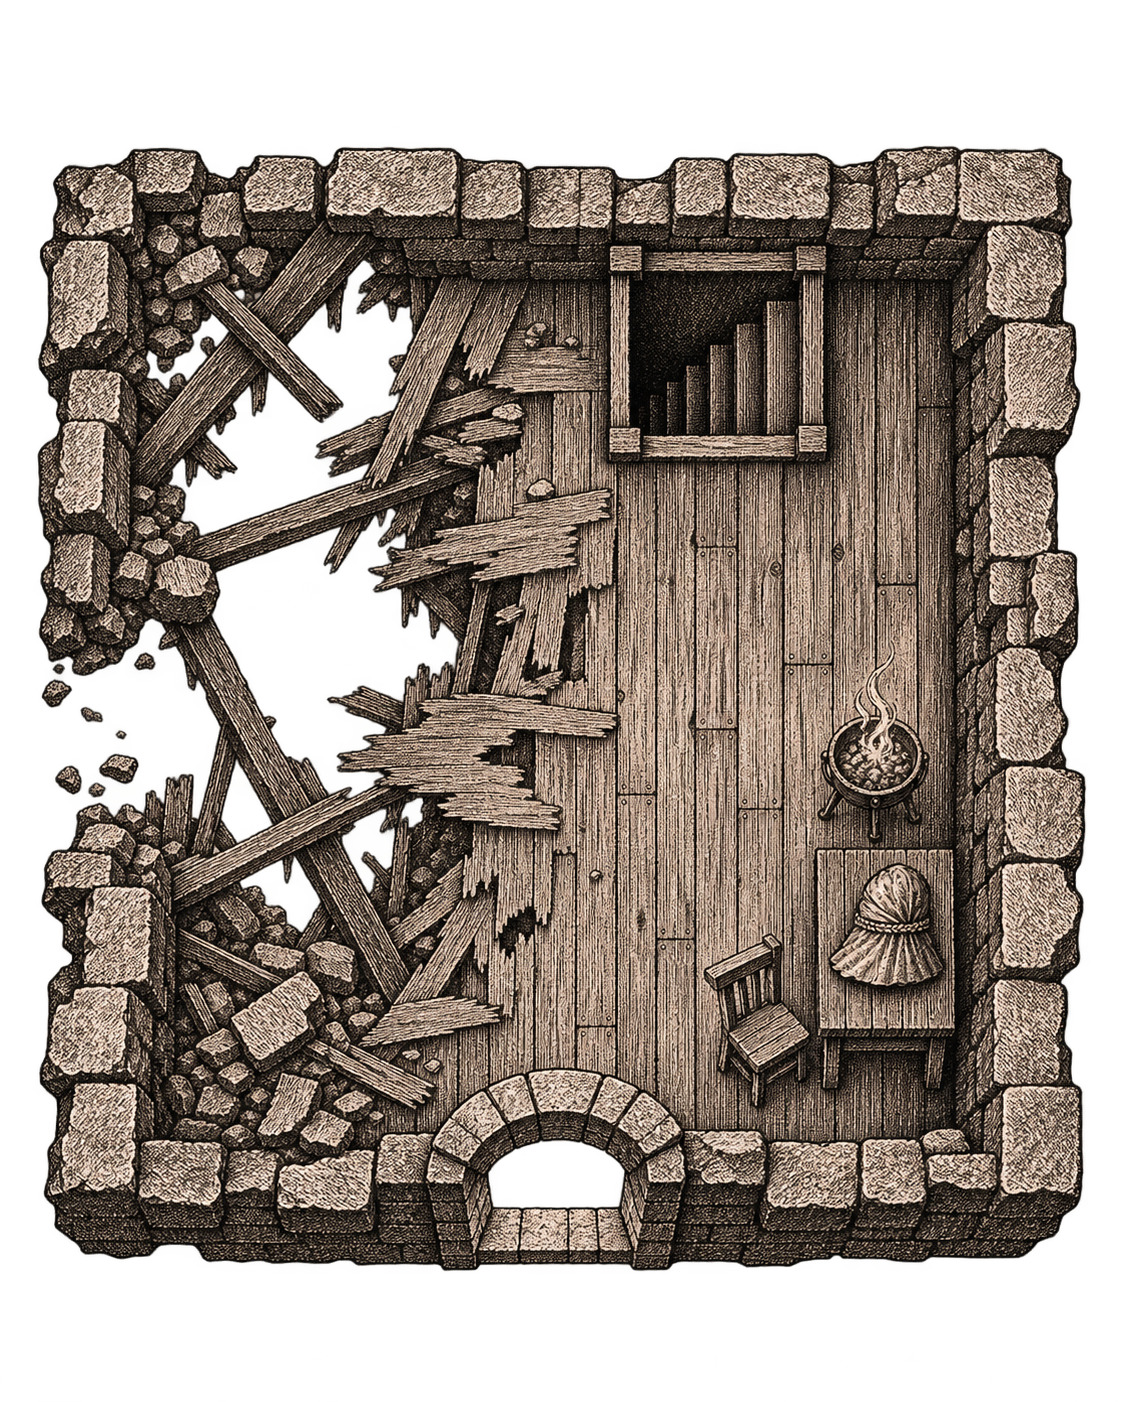
\includegraphics[width=.98\linewidth,height=70mm,keepaspectratio]{assets/hollow-hearth/map-upper.jpg}\par\vspace{2pt}
{\footnotesize\itshape\color{rpgbrown}Old Watchtower: upper floor\par}
{\scriptsize North stairway; exposed western side; south window, bell and brazier on the intact east.\par}
&
\centering\vspace{0pt}
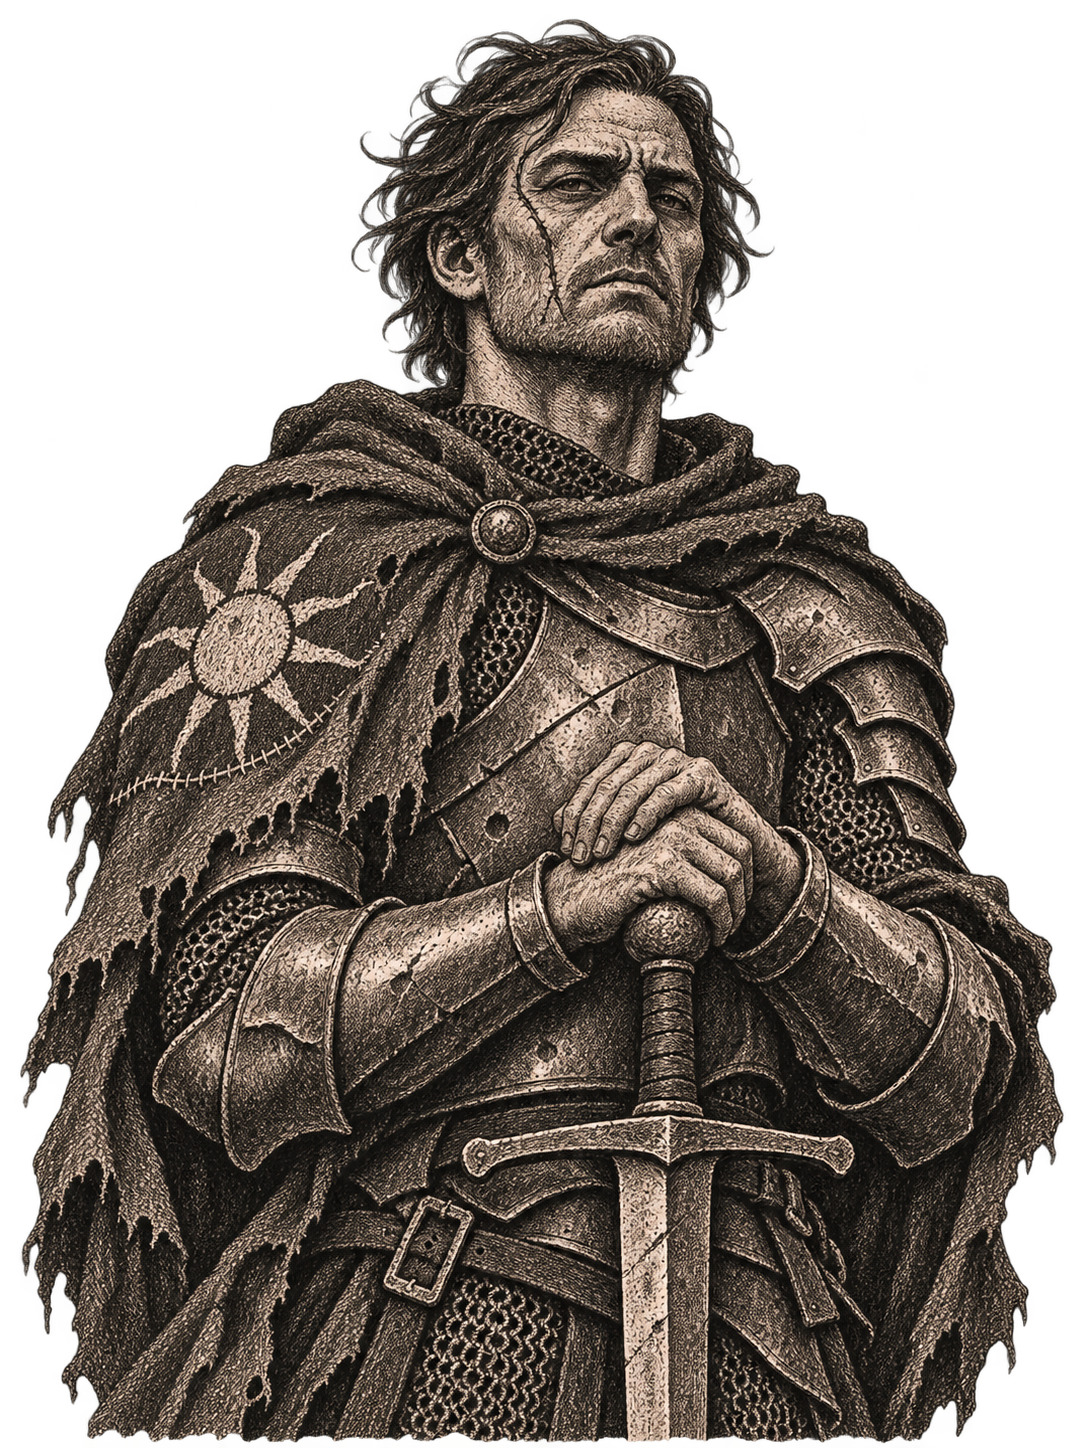
\includegraphics[width=.95\linewidth,height=68mm,keepaspectratio]{assets/hollow-hearth/corwin.jpg}\par\vspace{2pt}
{\footnotesize\itshape\color{rpgbrown}Sir Corwin Vask\par}
\end{tabular}
\par\medskip

Sir Corwin sits on a wooden chair beside the \textbf{south window}, watching the path the buyer will come up. The bell sits beside him on a small table, still wrapped in muddied oilcloth. A brazier of low coals provides the only warm light in the room. The stairs come up into the north wall --- \textbf{behind him}.

The \textbf{western half of the upper floor is open sky}: the same collapse that took out the western wall on the ground floor took out the western roof and part of the western flooring. Loose beams hang at angles. The exposed western flooring is unsafe to walk across without care.

This creates a \textbf{fourth approach} that the earlier text only hinted at:

\textbf{The Climb.} A character with \textbf{Acrobatics} can climb the rubble pile of the collapsed wall on the ground floor and continue up the outside of the broken western wall, entering through the gap in the roof. Roll \textbf{Dex + Acrobatics, TN 4} to climb cleanly; without Acrobatics, \textbf{TN 5}. A failure means falling --- 1 Wound from the height plus the noise of the fall (Corwin will hear). On a success, the character drops onto the upper floor \emph{behind} Corwin, with surprise. This is a single-character approach: the Fighter in heavy armour cannot make this climb, and the Mystic with 2 HP cannot afford the fall on a failure. \textbf{A nimble Adventurer is best suited to this approach.}

\par\Needspace{12\baselineskip}\noindent\textbf{Tactical features of the upper floor:}

\begin{itemize}
\tightlist
\item
  \textbf{The south window.} Anyone reaching the bell can hurl it out --- it lands hard near the campfire below, possibly cracked. The buyer, watching from the trail, will see it. A Protagonist can also use the window to escape the room, dropping to the ground (Dex + Acrobatics, \textbf{TN 4} to land cleanly; failure costs 1 Wound).
\item
  \textbf{The unsafe western half.} Combat that takes place on the collapsed half rolls under a Condition: \textbf{−1 tier}. A character forced over the edge falls one storey (2 Wounds). Corwin, who knows the room, will fight only on the eastern half --- and will gladly try to push enemies onto the bad footing.
\item
  \textbf{The brazier.} Tipped over, embers scatter onto the dry wood floor --- fire spreads in two scenes\textquotesingle{} worth of action, and the room becomes uninhabitable. A desperate move, available to anyone, that may save the party or destroy the bell along with everything else.
\item
  \textbf{Sir Corwin\textquotesingle s heavy armour.} His heavy armour sets the TN to hit him to \textbf{4 with Strength} or \textbf{5 with Dexterity}. It does not reduce damage. A tipped brazier, a push toward the collapsed edge, or a Critical from a Protagonist who declared Exertion can change the confrontation.
\end{itemize}

\subsubsection{Scaling the Encounter}\label{scaling-the-encounter}

\begingroup\setlength{\arrayrulewidth}{.34pt}\arrayrulecolor{rpgline}\renewcommand{\arraystretch}{1.32}\rowcolors{2}{rpgshade}{white}\par\smallskip\noindent\begin{tabularx}{\linewidth}{|Y|Y|Y}\hline
\rpghead{Party size} & \rpghead{Brigands} & \rpghead{Sir Corwin} \\ \hline
3 players & 3 brigands (group) & Yes \\ \hline
4 players & 4 brigands (2 outside, 2 inside) & Yes \\ \hline
\end{tabularx}\arrayrulecolor{black}\endgroup\par\smallskip

If the party seems to be struggling badly, have one brigand flee at the first sign of real bloodshed. If they are walking through it, the buyer arrives early.

\subsubsection{The Twist · The Buyer}\label{the-twist--the-buyer}

If the party is still at the watchtower at \textbf{midnight} --- whether mid-fight, talking, or having won --- a single robed figure walks out of the wood, alone, faceless under the hood. \textbf{The buyer is a Hollow person in mortal guise.} They want the bell silenced forever, not destroyed. They have a small bag of silver. They speak in the same not-quite-right voices the party half-heard on entering the wood.

\par\smallskip\begin{rpgnote}[fontupper=\normalfont]\textbf{The Buyer (Hollow Person in mortal guise)} \emph{TN S3/D4 · Expert · 4 Wounds · touch (1F Wonder; on Critical, 2W + a Condition that lasts the rest of the scene) · no armour.} \emph{Behaviour: "Speaks the wrong syllables. The trees do not answer. Bleeds sap, not blood."}\end{rpgnote}\par\smallskip
This is a \textbf{moment of choice}. The party can:

\begin{itemize}
\tightlist
\item
  \textbf{Refuse and fight.} \emph{(Stat block above.)}
\item
  \textbf{Accept the silver.} The party walks away rich. Hollow Hearth is not seen alive again. \emph{Let this be a real ending if they choose it.}
\item
  \textbf{Lie and ambush the buyer.} Opposed \textbf{Lore rolls vs the buyer\textquotesingle s Lore (Expert)}. If the party wins, they keep the silver \emph{and} the bell --- but the wood has marked them, and the next adventure begins with that mark.
\end{itemize}

\subsubsection{The Climax --- and the Last Throw}\label{the-climax--and-the-last-throw}

Whatever path is chosen, the climactic moment should leave at least one Protagonist in \textbf{Battered} or \textbf{Severe} state. Watch the HP totals at the table. The instant a player drops to \textbf{1 HP} and still has a roll to make to finish the scene --- pause. Look at them across the table. Ask:

\begin{quote}
\emph{"It\textquotesingle s at the last throw. Do you want to bleed for it?"}
\end{quote}

Walk them through declaring \textbf{Exertion} \emph{(manual p. 13)}. Let them roll; the Fatigue Wound comes after the roll. \textbf{This is the moment the game is named for.} Make it feel like it. If the roll succeeds, the room should cheer. If it fails, the room should fall quiet.

\par\vspace{3pt}

\subsection{Resolution}\label{resolution}

Three clean endings, with consequences that seed the next adventure:

\textbf{The Bell Returns.} Hesta awards the \textbf{Blade of Salt} and the village\textquotesingle s full hospitality. If her flower was brought back, Vela counts the party among her friends. Word spreads to the next town. \emph{The next adventure begins with the party being sought out by name.}

\textbf{The Bell is Silenced or Sold.} The party leaves rich and marked. The Hollow Folk note them. \emph{A future adventure begins with whispers in the night that know their names.}

\textbf{The Bell is Destroyed.} Whether by an unlucky Backlash or a desperate fight, the Hollow Folk return to Hollow Hearth on the moonless night. \emph{The next adventure begins with the party trying to undo it. Veyl Ashen, the original Mystic, may not be as dead as the histories say.}

\subsubsection{The Three Questions}\label{the-three-questions}

End the session by having the group answer the three Advancement questions together (manual p. 11). An honest accounting --- not a generous one --- is the right one. A new player who blocked at every turn earned no advancement points. A new player who tried, failed, and reckoned with consequence earned three. Make this clear, gently, the first time.

\par\vspace{3pt}

\par\smallskip\section*{Narrator's Quick Reference}\addcontentsline{toc}{section}{V. Narrator's Quick Reference}
\begingroup\footnotesize\setlength{\arrayrulewidth}{.34pt}\arrayrulecolor{rpgline}\renewcommand{\arraystretch}{1.14}
\noindent\begin{minipage}[t]{.49\linewidth}
\begin{tabularx}{\linewidth}{|>{\hsize=.78\hsize}Y|>{\hsize=1.22\hsize}Y|}\hline
\rpghead{Situation} & \rpghead{Rule / target} \\ \hline
TN 3–6 & Simple / Standard / Hard / Extreme \\ \hline
Distances & Close; Near; In Range; Far \\ \hline
Helping & Expert+: +1d6; below: +1d6 and TN +1 \\ \hline
Exertion & +1d6 before roll; 1F after \\ \hline
State & $\le$ 2 HP: $-1$ tier; $\le$ 1 HP: $-2$ tiers \\ \hline
\end{tabularx}
\end{minipage}\hfill
\begin{minipage}[t]{.49\linewidth}
\begin{tabularx}{\linewidth}{|>{\hsize=.78\hsize}Y|>{\hsize=1.22\hsize}Y|}\hline
\rpghead{Situation} & \rpghead{Rule / target} \\ \hline
Bridge & Dex TN 4; rope TN 3; fall 2W \\ \hline
Tracking & Dex + Survival, TN 4 \\ \hline
Stealth & Dex + Stealth, TN 4 \\ \hline
Climb & Dex + Acrobatics, TN 4 (else 5) \\ \hline
Corwin & TN S4/D5; Expert; 6W; sword 2W \\ \hline
\end{tabularx}
\end{minipage}
\arrayrulecolor{black}\endgroup


\HHAdventureBackCover
\end{document}
